\label{sec:signal}
This analysis searches for the simultaneous production of two massive bosons and a photon in a single hard scattering of a proton-proton collision at 13\TeV.
The signature of these processes varies among the three channels, but includes a number of high-momentum, isolated leptons,
with one or two pairs resonating to the Z boson mass,
and an isolated photon with high momentum.

The massive bosons are not stable particles and the most simple process that includes the VV\PGg production is 2 fermions $\to$ 4 fermions + a photon.
All Feynman diagrams with the same perturbative order, the minimal case being $\text{O}(\alpha_{EW}^5)\times\text{O}(\alpha_{QCD}^0)$,
must be taken into account in the generation of the signal process,
resulting in a certain degree of ambiguity in what can be considered triboson production when a photon is present in the final state.
We can classify the diagrams into three classes:

\begin{enumerate}
\item The photon is radiated from an initial state fermion (Figure \ref{fig:ppTo4LG_hard}), a case that includes Initial State Radiation (ISR) diagrams.
\item The photon emerges from a Triple or Quartic Gauge Coupling (e.g. Figure \ref{fig:ppTo4LG_GC}).
\item The photon is emitted as Final State Radiation (FSR) by one of the leptons from the decay of a vector boson (e.g. Figure \ref{fig:ppTo4LG_FSR}).
\end{enumerate}
Arguably, only the first and second process are strictly considerable triboson production.

The goal of this analysis is to measure both the cross sections and the significance of the inclusive processes
$pp \to 4\Pl \PGg$, $pp \to 3\Pl \PGnl \PGg$ and $pp \to 2\Pl 2j \PGg$
and of triboson production
in a region where diagrams of che classes 1 and 2 are enhanced.
Therefore a dedicated cut %% , described in Section \ref{sec:FSR_cut},
was devised to suppress events in which the (genuine) photon comes from final state radiation,
and results are derived both with (\textbf{triboson fiducial region}) and without (\textbf{inclusive cross section region}) applying it.

It is worth noting that in the SM only $\PW\PZ\PGg$ can be produced via triple and quartic gauge couplings,
while $\PZ\PZ\PGg$ does not have any leading order (perturbative expansion up to $\alpha_{EW}^5$) contribution from TGC nor QGC.

\begin{figure}
  \centering
  \subfigure [From initial-state fermion] {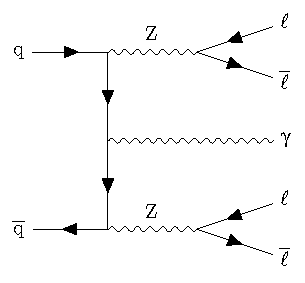
\includegraphics[width=.319\textwidth]{triboson_4LG.pdf} \label{fig:ppTo4LG_hard}}
  \subfigure [Non-abelian coupling]       {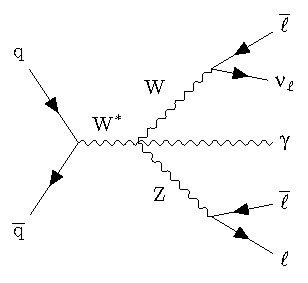
\includegraphics[width=.319\textwidth]{QGC_3LNuG.pdf}    \label{fig:ppTo4LG_GC}  }
  \subfigure [From final-state fermion]   {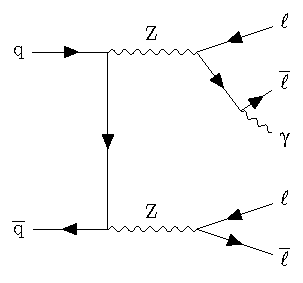
\includegraphics[width=.319\textwidth]{ZZ_4LG.pdf}       \label{fig:ppTo4LG_FSR} }
\caption{Representative Standard Model Feynman diagrams that yield four isolated leptons and a photon in the final state.}
\label{fig:ppTo4LG}
\end{figure}

\subsection{Signal definition}
\label{sec:signal_definition}
% the signal definition at gen level
The fiducial phase space definition mimics the selection applied to reconstructed events, described in Section \ref{sec:event_selection}.

The charged leptons, either electrons or muons are required to have $\pt > 5 \GeV$ and $|\eta| < 2.5$.
Each lepton pair $\Pl_i, \Pl_j$ must be separated $\DR(\Pl_i, \Pl_j) > 0.02$.
\todo{Is this actually done?}
Lepton isolation is ensured by requiring the scalar sum of the \pt of all stable particles, i.e.,
those particles not decaying in the detector volume, within a cone of radius $\DR = 0.3$ to be less than 0.35 times the \pt of the lepton.
\todo{Again, to be checked.}
Neutrinos, FSR photons, and leptons (electrons and muons) are not included in
the computation of the isolation sum to enhance the model independence of the measurements,
following the findings of Reference \cite{HIG-14-028}.
Low mass resonances are excluded by requiring that any opposite-sign lepton pair, regardless of flavour,
satisfies $m_{\Pl^{+} \Pl'^{-}} > 4\GeV$.

The number of charged leptons that pass these requirements is used to categorise the event into one of the three channels: 4\Pl, 3\Pl and 2\Pl.

The photon is required to have $\pt > 20 \GeV$, $|\eta| < 2.4$ and be produced in the hard scattering. % isPrompt
It must be separated from any lepton by $\DR(\PGg, \Pl) > 0.5$.
In all channels it is required the presence of a photon passing these requirements.

Jets are built with the \antikt algorithm with a distance parameter of 0.4,
and are required to have $\pt^{\rm jet} > 30 \GeV$ and $|\eta^{\rm jet}| < 4.7$, as done at the reconstruction level.
The jets are kept if no lepton or photon inside a cone with the size of the jet radius is found.
Large radius jets are built using a distance parameter of 0.8
and are required to have $\pt^{\rm jet} > 150 \GeV$ and $|\eta^{\rm jet}| < 4.7$.

In the 4\Pl channel the leading (sub-leading) lepton must have $\pt > 20\ (10) \GeV$.
There must be two pairs of same-flavour and opposite-sign (SFOS) leptons, which are labelled $\PZ_1$ and $\PZ_2$,
the former being the one with the mass closest the the Z peak, which must have $60 \GeV < m_{\PZ_{1,2}} < 120 \GeV$.

In the 3\Pl channel, the SFOS pair with the mass closest to the \PZ peak is selected first, and the remaining lepton is assigned to the \PW.
The mass of the \PZ boson must be $60 \GeV < m_\PZ < 120 \GeV$. %within 15 \GeV from the \PZ peak.
The leading (sub-leading) lepton from the \PZ boson must have \pt > 20 (10) \GeV,
while the lepton from the \PW must have \pt > 20 \GeV.
The transverse momentum of the neutrino is required to be larger than 30\GeV.

In the 2\Pl channel the two leptons must have same flavour and opposite sign
and the leading (subleading) lepton must have $\pt > 20\ (10) \GeV$.
There must be two jets with a mass such that $50\GeV < m_{jj} < 120\GeV$
or a single large radius jet with a mass in the the same range.

%% NOTE: The following paragraph is wrong
%% In the 2 \Pl channel, the two quarks from the decay of the VB must have $\pt > 30 \GeV$ and $|\eta| < 4.7$.
%% Their flavour must be compatible with a \PZ decay (e.g. \PQu\PAQu, \PQd\PAQd, \PQs\PAQs, \PQc\PAQc or \PQb\PAQb),
%% or a \PW decay (e.g. \PQu\PAQd, \PQu\PAQb, \PQd\PAQu, \PQd\PAQc, \PQs\PAQd or \PQs\PAQc).
%% The separation between the quarks and the photon must be $\DR(\PGg, \PQq) > 0.4$.


